\pdfoutput=1
% REPORT-001. Authoritative manuscript. Build with pdfLaTeX, twice (arXiv-compatible).
% Historical measurements are transcribed from recorded outputs of the manifest
% test scripts; this manuscript build does not rerun inference or constitute a new experiment.
\documentclass[11pt,a4paper]{article}
\usepackage[margin=23mm]{geometry}
\usepackage[T1]{fontenc}
\usepackage[utf8]{inputenc}
\usepackage{lmodern}
\usepackage{CJKutf8}
\usepackage{microtype}
\usepackage{amsmath,booktabs,array,graphicx}
\usepackage{tikz}
\usetikzlibrary{arrows.meta,positioning}
\usepackage[hidelinks]{hyperref}
\pagestyle{plain}
\setlength{\parindent}{1em}
\setlength{\parskip}{3pt}
\setlength{\emergencystretch}{1.5em}
\hypersetup{pdftitle={Echo: Composing Second-Language Replies by Steering a Conversation Model Word by Word},pdfsubject={Technical report; interaction design, implementation, and historical engineering measurements}}
\newcommand{\code}[1]{\texttt{#1}}
\newcommand{\zh}[1]{\begin{CJK}{UTF8}{gbsn}#1\end{CJK}}
\title{\vspace{-1.1cm}\textbf{Echo: Composing Second-Language Replies by\\Steering a Conversation Model Word by Word}\vspace{-0.2cm}}
\author{Yuxuan Chen\\
\small Ningbo University of Technology \quad $\cdot$ \quad \href{mailto:cyx3705@outlook.com}{\texttt{cyx3705@outlook.com}}}
\date{\vspace{-0.8em}\small Technical report \quad $\cdot$ \quad October 2026}
\begin{document}
\maketitle
\thispagestyle{empty}
\begin{abstract}
Second-language learners often recognize far more words than they can produce, yet AI writing aids tend either to leave them alone with a blank input box or to write the reply for them. Echo, a local prototype for Chinese-speaking learners of English, explores a middle ground in which the learner acts as the decoder. The same conversation model that plays the learner's partner continues the learner's own unfinished turn, and the interface presents its next-word distribution as a short list of glossed candidates. The learner either accepts one or types freely, so the reply is built one learner-chosen step at a time along the model's continuation tree, and nothing enters the text without a learner action. The loop also covers what the learner cannot yet say: a Chinese word typed in place is replaced by an English dictionary candidate selected in context. It also covers what the learner reads: partner replies carry per-word Chinese glosses chosen from dictionary senses, hidden once the learner marks a lemma as known and visibly marked when the system falls back to a default. The loop is only usable if candidates arrive before the next keystroke. Echo therefore reads the next-word ranking from a single forward pass over the learner's open turn and reuses the previous keystroke's KV state. On one laptop GPU this took a median of 5\,ms per keystroke, with every request under 100\,ms. A typical prompt-engineering alternative instead asks the same model through its API for ``the five words the learner is most likely to type next''. It took 364\,ms per keystroke, never returned within the 239\,ms mean inter-key interval of typists, and only 1.7 of its 5 words fit what had been typed. The same runtime puts all dictionary-bounded glosses of a partner reply on screen in 2.6\,s, compared with 7.5\,s through the API. No user study has been conducted; we state the hypotheses the design raises and outline how to test them.
\end{abstract}

\section{Introduction}
Producing a full English sentence can be difficult even when a learner recognizes most of the words it needs. Two common forms of AI support sit at opposite ends. A blank input box with an optional grammar checker leaves the production problem untouched. A system that drafts or rewrites the whole reply removes the problem, and with it most of the learner's own production. Echo explores the space between them.

In Echo, the learner converses in English with a local language model. While the learner composes, the \emph{same} model, with the same conversation history and instruction, is asked to continue the learner's unfinished turn. Its ranked next-word predictions are shown as a few candidates, each with a short Chinese gloss. The learner can accept one, keep typing, or edit. In effect the learner replaces the sampler of a conversational language model: each acceptance commits one branch of the model's continuation tree, chosen by a person with something to say rather than by a random draw. When a word is missing entirely, the learner can type it in Chinese and let Echo choose a matching English dictionary entry in context. When reading the partner's reply, the learner sees Chinese glosses for words not yet marked as known.

This report makes five contributions:
\begin{itemize}\setlength{\itemsep}{1pt}
\item \textbf{An interaction paradigm} for second-language conversation in which the learner steers a conversation model's prediction of the learner's own turn, one word at a time, with comprehension support for the partner's turn in the same dialogue (Section~\ref{sec:paradigm}).
\item \textbf{A concrete design} of that loop and its rationale: glossed candidates, partial-word handling, in-place Chinese-to-English lookup, a lemma-level ``known'' state that removes glosses, and visible marking of uncertain glosses (Section~\ref{sec:design}).
\item \textbf{A single-GPU implementation} that keeps prediction and gloss selection responsive by sharing one model's computed context and restricting model output to dictionary choices (Section~\ref{sec:implementation}).
\item \textbf{A latency evaluation against HCI thresholds}: per-keystroke next-input prediction compared with the same model queried through an API, both with the same one-pass formulation and with prompt engineering. It shows that the formulation decides between usable and unusable, and that shared KV adds headroom. Glossing and lookup are compared as well, including the case where the API is faster (Section~\ref{sec:results}).
\item \textbf{A research agenda}: the hypotheses that a user study would need to test (Section~\ref{sec:limitations}).
\end{itemize}
Model-guided text entry, predictive keyboards, and human--AI co-writing all have established predecessors (Section~\ref{sec:related}). We make no claim of being first. What we contribute is the combination of learner-steered decoding of one's own turn, the second-language setting, and comprehension support within a single conversational loop.

\section{Interaction paradigm: the learner as decoder}
\label{sec:paradigm}
Let $h$ be the conversation so far, $s$ the partner's system instruction, and $u_{<t}$ the learner's unfinished message. Echo renders $h$ with the model's own chat template and leaves the learner's turn \emph{open}, ending at $u_{<t}$, so that the model's next-token distribution $p_\theta(\cdot\mid s,h,u_{<t})$ is a prediction of what the learner will say next. Generating from this distribution would let the model speak for the learner. Echo instead exposes a filtered top-$k$ of it, and the learner chooses:
\begin{equation}
 u_t \in \mathrm{Filter}_k\!\left(\operatorname{top20} p_\theta(\cdot\mid s,h,u_{<t})\right)\;\cup\;\{\text{anything the learner types}\}.
\end{equation}
The candidates come from the partner's own context. They therefore reflect the topic and the partner's last question. Each acceptance appends a word and immediately requests the next ranking, so a reply is a path through the model's continuation tree, walked one level at a time by the learner. Echo does not display the tree itself. It shows only the current level's alternatives, which keeps the choice small and keeps the learner reading forward rather than browsing completions.

\begin{figure}[ht]
\centering
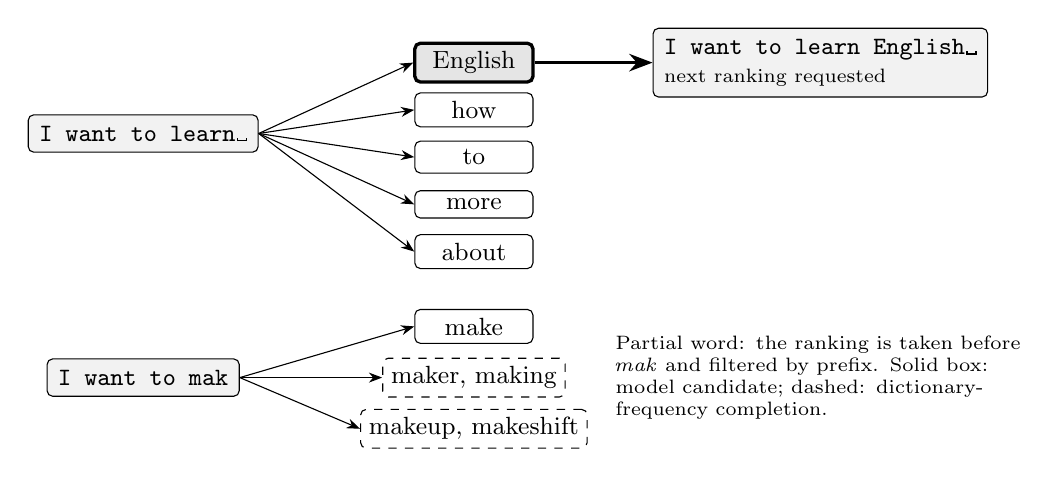
\begin{tikzpicture}[font=\small,>=Stealth,
 ctx/.style={draw,rounded corners=2pt,fill=black!5,align=left,inner sep=4pt},
 cand/.style={draw,rounded corners=2pt,inner sep=3pt,minimum width=15mm,align=center},
 pick/.style={cand,very thick,fill=black!10}]
\node[ctx] (c1) at (0,0) {\code{I want to learn\textvisiblespace}};
\node[pick] (k11) at (4.2,0.9) {English};
\node[cand] (k12) at (4.2,0.3) {how};
\node[cand] (k13) at (4.2,-0.3) {to};
\node[cand] (k14) at (4.2,-0.9) {more};
\node[cand] (k15) at (4.2,-1.5) {about};
\foreach \k in {k11,k12,k13,k14,k15} \draw[->] (c1.east) -- (\k.west);
\node[ctx] (c2) at (8.6,0.9) {\code{I want to learn English\textvisiblespace}\\[-1pt]{\scriptsize next ranking requested}};
\draw[->,very thick] (k11.east) -- (c2.west);
\node[ctx] (c3) at (0,-3.1) {\code{I want to mak}};
\node[cand] (m1) at (4.2,-2.45) {make};
\node[cand,dashed] (m2) at (4.2,-3.1) {maker, making};
\node[cand,dashed] (m3) at (4.2,-3.75) {makeup, makeshift};
\foreach \k in {m1,m2,m3} \draw[->] (c3.east) -- (\k.west);
\node[align=left,font=\scriptsize,text width=52mm] at (8.6,-3.1) {Partial word: the ranking is taken before \emph{mak} and filtered by prefix. Solid box: model candidate; dashed: dictionary-frequency completion.};
\end{tikzpicture}
\caption{Two recorded candidate lists (\code{qwen3:8b}, five candidates; 23 October 2026). Top: the learner accepts \emph{English} with Shift+Space (an illustrative choice), and the next level is requested at once. Each displayed candidate also carries a short Chinese dictionary gloss, omitted here.}
\label{fig:walk}
\end{figure}

Three properties distinguish this from the most common forms of AI writing support. First, \emph{nothing enters the message without a learner action}: there is no auto-completion of whole phrases or replies, and the learner can ignore candidates entirely. Second, the predictions come from the \emph{conversation partner's} context rather than from a general keyboard model or a separate tutor model. Third, each step is a lexical decision the learner can inspect, since the candidate shows the word and a gloss. The intended effect is to turn production into a sequence of recognition decisions while keeping the learner in charge of meaning. Whether this helps or hinders learning is an empirical question that this report does not answer (Section~\ref{sec:limitations}).

\section{Design}
\label{sec:design}
Five working principles guided the design:
\textbf{(D1)} learner agency: the model proposes and the learner commits;
\textbf{(D2)} bounded model output: Chinese shown to the learner comes from a dictionary, never from free-form generation;
\textbf{(D3)} honest uncertainty: a fallback gloss is visibly marked;
\textbf{(D4)} attention economy: words the learner knows stop receiving support;
\textbf{(D5)} responsiveness: candidates must keep pace with typing on one consumer GPU.

\subsection{Composer}
One forward pass yields a top-20 next-token ranking. Echo keeps space-prefixed English words that have a dictionary entry (single letters only \emph{a} and \emph{I}) and four punctuation marks, removes duplicates case-insensitively, and displays up to the configured number (five by default, 1--20). Each candidate shows its number, the word, and a short Chinese gloss. Shift+W and Shift+S move the selection, and Shift+Space accepts it (Tab and clicking also accept). Ordinary Space types a space and Enter sends, so free typing is never intercepted (D1). Accepting appends the word and a space and requests the next ranking. At the start of a turn only capitalized candidates are kept, because lower-case turn-initial tokens are mostly word fragments. A partial word is never fed to the model, since prompts cut inside a token produced misspellings such as \emph{makng}. Echo ranks before the word, filters by the typed prefix, and completes from dictionary frequency when the model offers too few (Figure~\ref{fig:walk}). The candidate row keeps a fixed height while it updates, so the input box does not jump. Dictionary membership cannot prove that a token ends a word: multi-token words may be missed and fragments shown.

\subsection{Saying what you cannot yet say in English}
\label{sec:reverse}
While Ctrl is held, a native child control embedded in the composer hosts the system Chinese input method. Releasing Ctrl writes the committed Chinese back at the cursor. An ordinary Space then confirms the preceding run of Chinese, possibly typed over several Ctrl sessions, as one word of 1--32 characters. Echo looks it up in reverse in an English--Chinese dictionary (up to 20 words or phrases) and lets the model choose among them from the conversation and the text around the word. The chosen entry replaces the Chinese in place. If there is no entry, or the model abstains, the Chinese stays (D2): Echo never falls back to a free-form translation. Examples include \zh{苹果}$\to$\emph{apple} and \zh{冰淇淋}$\to$\emph{ice cream}; Section~\ref{sec:results} reports the measured latency. While the request runs, prediction and sending pause, but editing remains possible. A stale result never overwrites later edits.

\subsection{Reading the partner's turn}
Partner replies stream in English with a small Chinese gloss under each word. A word with a single dictionary sense is glossed directly. For an ambiguous word, the model chooses among that word's dictionary senses, or abstains, using only the conversation up to that word, never text the partner has not yet produced. The choice streams in as the reply continues. If selection abstains, overflows its bounded queue, times out, or fails, Echo shows a deterministic dictionary default with an underline, and hovering reveals the reason (D3). The underline marks a recognized fallback. It does not detect all wrong meanings, so a confidently wrong gloss can remain unmarked. Clicking a word marks its lemma as known (\emph{went} marks \emph{go}). Its glosses are then hidden everywhere while their space is kept, so the layout does not reflow, and Echo stops computing glosses for that lemma altogether (D4). Learned state is stored locally and is shared with a browser extension that applies the same glossing to webpage text. There, visible text is supplied in chunks of about 600 characters, so a webpage gloss may use later text in the same chunk.

\section{Making the loop responsive}
\label{sec:implementation}
Echo 0.3.0 is a local FastAPI service with a browser UI. Python handles HTTP/SSE transport, prompts, dictionary access, learned state, and orchestration. A C++ runtime built on llama.cpp~\cite{llamacpp} handles tokenization, KV state, batching, sampling, next-token ranking, constrained selection, and branch cleanup. It runs one quantized 8B model (\code{qwen3:8b}) in one fixed 4,096-token KV pool with three sequence slots, and never loads a second model. Ollama supplies model management and the bundled llama.cpp library, which Echo's adapter loads directly because the HTTP interface does not expose live sequence handles. The dictionary is ECDICT~\cite{ecdict}.

\paragraph{Incremental prediction (D5).} The runtime keeps the KV state and ranking of the most recent prediction in an idle slot. When the prompt changes, it reuses the longest common \emph{token} prefix and computes only the changed tail. An identical prompt reuses the stored ranking without a forward pass. Frontend scheduling uses a 25\,ms debounce, one in-flight request, and only the latest pending input. Starting a partner reply clears this cache.

\paragraph{Finite-choice selection (D2).} All three model choices that the learner sees as Chinese or English text (partner glosses, webpage glosses, and Chinese-to-English replacement) take the same form. Let $P$ be an already computed prefix, $S_i$ a short task suffix for item $i$, and $D_i$ its dictionary entries. Each entry receives a label, plus an abstention label $0$. The runtime picks
\begin{equation}
 \hat{\ell}_i = \arg\max_{\ell\in\mathcal L_i} z_\theta(\ell\mid P,S_i),\qquad
 g_i = \begin{cases}D_i[\hat{\ell}_i],&\hat{\ell}_i\ne0,\\ d_i^{\mathrm{default}} \text{ (marked) or no change},&\hat{\ell}_i=0,\end{cases}
\end{equation}
where $z_\theta$ is the next-token logit restricted to allowed labels. The dictionary, not generated text, supplies $g_i$. Webpage glosses and Chinese-to-English replacement use single-token letter labels (A--Z and a--z, or A--T), so one output decision suffices however long the gloss or phrase is. Partner glosses constrain decoding to the Chinese sense strings through a token trie, stopping at the first token that identifies a unique sense (at most 16 decisions and a 640-token task). During development, letter labels mis-selected a sense of \emph{dishes} on this path. Logits are not calibrated probabilities. Prompt prefill still costs time, so ``one decision'' never means one GPU call per request.

\paragraph{Shared context.} A partner-gloss task must see the conversation exactly up to the target word while the partner keeps generating. The runtime therefore forks a short-lived branch that references the partner's \emph{actually computed} KV prefix through that word (\code{llama\_memory\_seq\_cp}). If the word ends inside a token, the branch starts at the preceding valid token boundary and recomputes only the remainder. The branch then closes the turn with the model's template tokens, appends the task, takes its decision, and is released at once (Figure~\ref{fig:architecture}). At most one such branch is live, and pending work is bounded to eight lightweight descriptions; overflow falls back. Branch prefill yields every 64 tokens so the partner keeps streaming. Native locking preserves the partner's pending sample and logits. Webpage text is prefilled once as input, and two occurrence-specific branches share that prefix in one native batch. Branch suffixes are limited to 640 tokens each and 704 combined. Each branch and source is released on success, failure, or cancellation. Releasing makes pool space reusable but need not reduce preallocated VRAM.

\begin{figure}[ht]
\centering
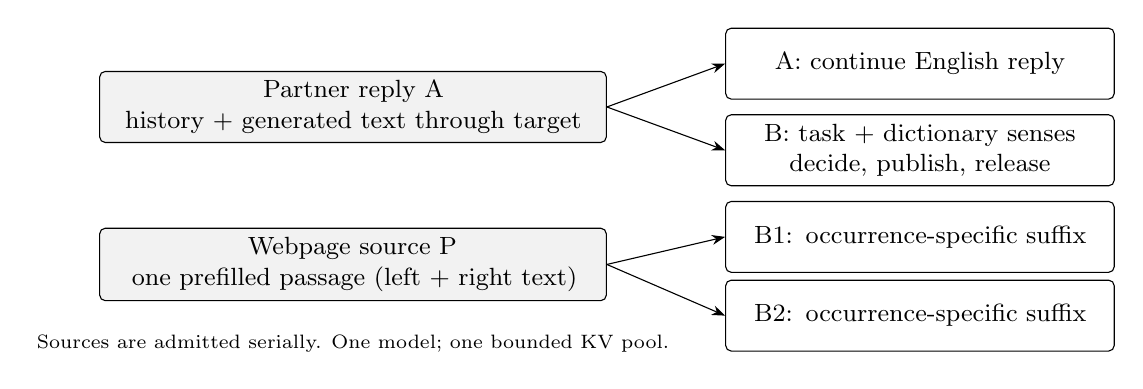
\begin{tikzpicture}[font=\small,>=Stealth,
 box/.style={draw,rounded corners=2pt,align=center,minimum height=9mm,text width=47mm},
 base/.style={box,fill=black!5,text width=62mm}]
\node[base] (a) at (0,0) {Partner reply A\\history + generated text through target};
\node[box] (ac) at (7.2,0.55) {A: continue English reply};
\node[box] (b) at (7.2,-0.55) {B: task + dictionary senses\\decide, publish, release};
\draw[->] (a.east) -- (ac.west);
\draw[->] (a.east) -- (b.west);
\node[base] (p) at (0,-2.0) {Webpage source P\\one prefilled passage (left + right text)};
\node[box] (b1) at (7.2,-1.65) {B1: occurrence-specific suffix};
\node[box] (b2) at (7.2,-2.65) {B2: occurrence-specific suffix};
\draw[->] (p.east) -- (b1.west);
\draw[->] (p.east) -- (b2.west);
\node[align=center,font=\scriptsize] at (0,-3.0) {Sources are admitted serially. One model; one bounded KV pool.};
\end{tikzpicture}
\caption{Gloss branches share their source's computed KV prefix. A partner-gloss branch cannot read later reply text; webpage branches can read the whole supplied passage. Chinese-to-English replacement uses one short-lived source and branch.}
\label{fig:architecture}
\end{figure}

\section{Evaluation: is next-input prediction fast enough to be usable?}
\label{sec:results}
The paradigm stands or falls with prediction speed. A candidate list is useful only if it reflects what the learner has just typed. If it arrives after the next keystroke, it describes text that no longer exists, and it still costs attention to read~\cite{quinn}. We therefore compare ways of predicting the learner's next input against latency limits from the HCI literature, using the same model, inputs, and hardware.

\subsection{Latency budget}
Classic guidance holds that about 0.1\,s is the limit for a response to feel instantaneous, and about 1\,s the limit for keeping the user's flow of thought~\cite{nielsen,miller,card}. For typing, the relevant clock is the inter-key interval. In 136 million keystrokes from 168,000 volunteers, the mean interval was 239\,ms. It was about 122\,ms for the fastest typists and 481\,ms for the slowest~\cite{dhakal}. Second-language learners composing a message are likely nearer the slow end, but they still type several characters per second. We therefore treat a prediction as usable for a keystroke if it is ready within 239\,ms, and as comfortably usable if it is ready within 100\,ms. Above 481\,ms it is stale even for slow typists.

\subsection{Methods compared}
All three methods use the same \code{qwen3:8b} weights, the same partner system instruction, and a 12-turn conversation history. Each sends one request per input change, as Echo does, with no parallel fan-out of requests.
\begin{itemize}\setlength{\itemsep}{1pt}
\item \textbf{Echo (one pass, shared KV).} The learner's turn is left open and the next-token ranking is read from a single forward pass, reusing the KV state of the previous keystroke (Section~\ref{sec:implementation}). The ranking is then filtered through the dictionary.
\item \textbf{One pass through the API.} The same formulation through the HTTP API of the Ollama engine bundled with Echo: one generated token with its top-20 log-probabilities. Ollama's own prompt cache is enabled.
\item \textbf{Prompt engineering through the API.} This is what a typical LLM application would do. A chat request asks the model, in the same conversation, for \emph{``the 5 words the learner is most likely to type next''} (or completions of a partial word), and a JSON schema constrains the reply to five strings.
\end{itemize}
The main workload types one learner message, \emph{``I would like to visit a quiet park with my friends.''}, character by character after 12 dialogue turns: 51 input changes, repeated five times. Four shorter word-level sequences from the earlier record were also run. A candidate counts as valid if it is a single dictionary word (or one of four punctuation marks) consistent with any partial word typed. Timings are client-side on loopback and exclude Echo's 25\,ms debounce and rendering. The two conditions ran one after the other on 25 October 2026 (only one model copy fits in 12\,GB VRAM), with other GPU applications open.

\begin{table}[ht]
\centering\footnotesize\setlength{\tabcolsep}{4pt}
\begin{tabular}{@{}lrrrrr@{}}
\toprule
 & \multicolumn{3}{c}{Per keystroke, 12-turn history (250 requests)} & Word-level & Valid\\
\cmidrule(lr){2-4}
Method & p50 / p95 & $\le$100\,ms & $\le$239\,ms & p50 range & of 5\\
\midrule
Echo: one pass, shared KV & \textbf{5.1} / 21.2\,ms & 100\% & 100\% & 4--20\,ms & 4.76\\
One pass through the API & 27.9 / 36.0\,ms & 100\% & 100\% & 24--29\,ms & 4.76\\
Prompt engineering through the API & 364 / 651\,ms & 0\% & 0\% & 345--381\,ms & 1.69\\
\bottomrule
\end{tabular}
\caption{Next-input prediction, same model, inputs, and machine (25 October 2026). Keystroke columns exclude the first request of each repetition. ``Valid'' is the mean number of usable candidates out of five on the per-keystroke workload; the prompt-engineering method gave 2.5--3.2 on the word-level sequences. At most 84\% of its keystroke requests finished within the slow-typist interval of 481\,ms.}
\label{tab:prediction}
\end{table}

\paragraph{Usable versus unusable.} The prompt-engineering method never returned within the 239\,ms of an average keystroke, and it took 364\,ms at the median. By the time its list appeared, the learner had typed one or two further characters. Its words often did not fit what had been typed: on average only 1.7 of 5 were valid, because a chat model asked to ``predict the next words'' tends to answer with whole phrases, repeat what was typed, or ignore a partial word. Asking for candidates in parallel would not help, because each request would still generate a reply. Both one-pass methods returned every request within 100\,ms with valid candidates, and they produce the same candidate lists up to small numerical differences, because they read the same ranking. The decisive step is therefore the formulation of prediction itself. Reading the model's next-token distribution over the learner's own open turn replaces a generated answer with a single forward pass.

\paragraph{What shared KV adds.} Keeping the previous keystroke's KV state and ranking cut the median per keystroke from 28\,ms to 5\,ms. Inside a word, the stored ranking is reused without any model call. Both are already below perception thresholds on this GPU, so the extra margin matters in other ways. It leaves the GPU free for the partner's streaming reply and gloss branches. It leaves headroom for slower hardware and longer conversations. And it keeps the cost of each keystroke nearly independent of history length once the first request after a context change has been paid. That first request took 214--217\,ms with 12 turns of history in Echo. The API's first requests are not compared, because Ollama's prompt cache was not reset between repetitions.

\subsection{Glosses and Chinese-to-English lookup}
The same comparison was run for the reading side and for reverse lookup (Table~\ref{tab:comparison}). The API baseline streams the reply and, through Ollama's second slot, sends a structured request for each ambiguous word as soon as it is complete. The runtime instead forks a branch from the reply's computed prefix. The difference shows mainly in \emph{when} glosses appear. Through the API, the last gloss arrived about 6\,s after the English text was complete, so the learner would read most of the reply unaided. With the runtime, all glosses were on screen 2.6\,s after the request, several of them before the text finished. Free-form translation through the API was fast but unbounded: only 12 of 42 answers equalled a dictionary sense, some were explanations or translated the wrong word (\emph{dishes}$\to$\zh{洗碗}, ``wash dishes''), and none abstained. The accuracy gap between the runtime and the structured API path comes mainly from prompts and abstention policy, not from KV reuse. These cases were also used during prompt development. For Chinese-to-English lookup, a single user-triggered request, the API path was faster, because the runtime must build a fresh source and branch. Prefix sharing brings no benefit there.

\begin{table}[ht]
\centering\footnotesize\setlength{\tabcolsep}{4pt}
\begin{tabular}{@{}llrrr@{}}
\toprule
Task & Measure & Runtime & API (constrained) & API (free-form)\\
\midrule
Gloss for an ambiguous word & latency p50 / p95 & 205 / 265\,ms & 707 / 793\,ms & 103 / 265\,ms\\
 & accepted answer & 42/42 & 30/42 & 24/42\\
 & output is a dictionary sense & 42/42 & 42/42 & 12/42\\
\addlinespace
Partner reply with glosses & English text complete & 1.42\,s & 1.31\,s & ---\\
 & all glosses on screen & 2.58\,s & 7.50\,s & ---\\
 & glosses before text ends & 3--4 of 9--10 & 0--1 of 9 & ---\\
\addlinespace
Chinese-to-English & latency p50 / accepted & 106\,ms / 15/15 & 46\,ms / 15/15 & 69\,ms / 15/15\\
\bottomrule
\end{tabular}
\caption{Glossing and reverse lookup, same model and machine (25 October 2026): 14 cases $\times$ 3, three replies, 5 words $\times$ 3. Three gloss cases encode Echo's policy of abstaining on insufficient left context; excluding them, the counts are 33/33, 30/33, and 24/33. Free-form answers are judged leniently and cannot abstain.}
\label{tab:comparison}
\end{table}

\paragraph{Caveats.} Each condition was run once, on one machine, with background GPU load and one model. Reply lengths vary with sampling. A cloud API would add network round trips to every keystroke and would send learner text off the device, which Echo avoids by design. The thresholds bound perceived latency only. Whether timely candidates help learners is the question of Section~\ref{sec:limitations}.

\subsection{Earlier engineering records}
The following observations come from recorded outputs of the repository's test scripts on 24 October 2026, under the same hardware and model. In an earlier prediction benchmark, incremental caching reduced subsequent-request medians from 54.8--227.8\,ms to 9.5--26.2\,ms. One request reused 851 tokens and evaluated one. Cached and cold GPU scores differ slightly (largest shared top-20 log-probability difference about 0.225), while reuse of an identical prompt's ranking is exact. For webpage glossing, four hand-written passages each contain two target occurrences: river and financial \emph{bank}, weight and illumination \emph{light}, noise and structural \emph{sound}, and reservation and printed \emph{book}. The test runs one-branch mode, then two-branch mode, for 16 target decisions over eight unique occurrences. All met the accepted-sense checks with one output decision each (Table~\ref{tab:reader}).

\begin{table}[ht]
\centering\small
\begin{tabular}{@{}lrr@{}}
\toprule
Passage targets & One branch (ms) & Up to two branches (ms)\\
\midrule
bank: \zh{岸} / \zh{银行} & 561.1 & 201.3\\
light: \zh{轻的} / \zh{光源} & 961.1 & 757.6\\
sound: \zh{声音} / \zh{健全的} & 472.8 & 410.4\\
book: \zh{预订} / \zh{书} & 254.9 & 209.2\\
\bottomrule
\end{tabular}
\caption{One recorded webpage run: time to finish all eligible glosses in each passage, not just its two targets. Initial dictionary events took approximately 1.5--8.6\,ms; input prefixes were 131--133 tokens. Serial test order introduces warm-state confounding, so these timings do not establish a batching speedup.}
\label{tab:reader}
\end{table}

\subsection{Lifecycle, isolation, and verification status}
A 1,000-cycle fork/release check took 23.93\,s and ended with zero active source and branch handles; cumulative fork and release counts both reached 1,016 including other checks. With a fixed seed (73), the partner's reply text was identical with and without short and long gloss branches inserted. In the same run, the reply's inter-token P50 was about 14\,ms alone, and its P95 was about 39\,ms with a long branch inserted, so glossing is not free for the partner's stream. These checks support lifecycle accounting and limited sampling isolation. They do not measure physical KV bytes or prove leak freedom or determinism for all workloads. An isolated Edge session exercised the Manifest V3 extension end to end, and fixture-based browser checks covered learned-state reversal, offsets, dynamic text, fallback marking, and DOM restoration. Chrome and arbitrary websites have not been validated. The latest recorded application regression had 54 of 55 Python tests passing. All 14 C++ inference groups passed, but the Windows \code{input\_tests.exe} process exited with code 3221226505 for an unresolved reason, so we do not describe the complete suite as passing.

\section{Related work}
\label{sec:related}
\paragraph{Language-model-guided text entry.} Dasher lets people write by steering through a space allocated in proportion to a language model's predictions~\cite{dasher}. It is the closest conceptual precedent for treating the person as the decoder. SpeakFaster uses large language models and conversational context to expand abbreviated input for eye-gaze typists with ALS~\cite{speakfaster}. Both aim at entry speed or accessibility for people who already know what they want to say. Echo applies the steering idea to a learner who is still forming the utterance in a second language. Its predictions come from the conversation partner's own context, and lexical support is shown at every step.

\paragraph{Response time.} Response-time limits for interactive systems have been stable since Miller's analysis of conversational transactions~\cite{miller}. About 0.1\,s feels instantaneous and about 1\,s preserves the flow of thought~\cite{card,nielsen}. Large-scale typing data put the mean inter-key interval near 239\,ms~\cite{dhakal}. Quinn and Zhai show that suggestions save keystrokes but cost attention, so suggestions that are late or wrong are worse than none~\cite{quinn}. Echo uses these figures as its design budget (Section~\ref{sec:results}).

\paragraph{Effects of suggestions on writing.} Predictive suggestions change what people write. Arnold et al.\ found that captions written with suggestions were shorter and more predictable~\cite{predictable}. Buschek et al.\ found that multiple parallel phrase suggestions aided ideation at a cost to efficiency, and that non-native writers appeared to benefit more from additional suggestions~\cite{parallel}. CoAuthor records human--AI co-writing sessions at scale~\cite{coauthor}. These results motivate both Echo's design, which offers several single-word options and lets the learner type freely at any point, and its central open risk: steering a learner towards predictable language.

\paragraph{Supporting techniques.} Gloss-based word-sense disambiguation is established~\cite{glossbert}, as are lexically constrained and grammar-guided decoding~\cite{hokamp,outlines} and shared-prefix KV reuse in serving systems~\cite{vllm,sglang,hydragen}. Echo uses these techniques and does not claim to advance them. Its specific requirement is local: on one consumer GPU, gloss branches must fork from a reply that is still being generated, at a past position, without slowing the conversation noticeably. Echo's branches are discarded after one choice and do not implement search over reasoning paths such as Tree of Thoughts~\cite{tot}.

\section{Limitations, hypotheses, and evaluation plan}
\label{sec:limitations}
\paragraph{No learner evidence yet.} This report documents a working system. It does not show that learners write better, learn vocabulary, feel more confident, or prefer Echo over ordinary predictive keyboards, dictionaries, or full-reply suggestions. A ``known'' flag records a learner's choice, not measured mastery.

\paragraph{Hypotheses.} The design raises testable questions:
\textbf{H1}, learner-steered word candidates let learners complete more and longer replies than free typing, while preserving more learner-originated content than full-reply suggestion;
\textbf{H2}, following the predictability effect~\cite{predictable}, candidate use reduces lexical diversity, and this effect depends on how many candidates are shown~\cite{parallel};
\textbf{H3}, glossed candidates and in-place Chinese-to-English replacement expose learners to new words that they later recognize at above-baseline rates;
\textbf{H4}, the visible fallback mark helps learners judge when a gloss is uncertain.

\paragraph{Evaluation plan.} A within-subjects study with Chinese-speaking learners at two proficiency levels could compare three composers in the same conversational tasks: free typing with a dictionary, Echo, and whole-reply suggestions. Production measures would be completion, length, and the proportion of typed versus accepted words. Language measures would cover lexical diversity, error rate, and similarity to the model's top-1 continuation. Experience measures would cover perceived agency and workload. A delayed recognition test of words first met through candidates or replacements would address H3. Logged interaction traces would allow suggestion-level analysis.

\paragraph{System limits.} Gloss quality is bounded by the dictionary, which may lack a phrase sense or split meanings poorly, and by the model's uncalibrated choice. Partner glosses are deliberately causal: at ``the bank'', later words could settle the meaning but the branch cannot see them. Webpage and replacement labels pair a bare \code{0} with space-prefixed letter tokens; project notes flag this tokenization asymmetry as a possible source of label bias, which has not been measured. The 16 webpage decisions are a smoke test, not an accuracy estimate. Candidate filtering cannot verify word boundaries, conversation templates are written per model family (Qwen and Gemma), the KV pool and queues are small and fixed, and the Chinese input bridge is Windows-specific and has an unresolved test failure.

\section{Reproduction and artifact scope}
\label{sec:reproduction}
The report describes Echo 0.3.0 at the working-tree inspection of 24 October 2026. It accompanies the implementation rather than claiming a public release or an immutable benchmark package. Tables~\ref{tab:prediction} and~\ref{tab:comparison} come from \code{b-Code-Echo/tests/api\_comparison.py}, run in both modes on 25 October 2026 (\code{-{}-predict-only} for Table~\ref{tab:prediction}). Table~\ref{tab:reader} and the other figures transcribe the JSON outputs of the repository's test scripts from earlier recorded runs. The project conventions document (\code{b-Office/}\zh{现行约定}\code{.md}) summarizes them, partly as rounded ranges, and records the candidate lists of Figure~\ref{fig:walk}. Re-running the scripts produces new observations, not the exact historical traces.

The native setup requires Windows x64, Python 3.12 or later, Visual Studio C++ Build Tools and the Windows SDK, the local model, and the ECDICT SQLite dictionary. With dependencies prepared and Echo running idle, the following repository-root commands invoke the relevant checks. GPU checks should run serially.
\begin{quote}\footnotesize\ttfamily
uv run -{}-project b-Code-Echo python\\
\hspace*{1em}b-Code-Echo/tests/native\_suggest\_performance.py -{}-repeats 5\\[3pt]
uv run -{}-project b-Code-Echo python\\
\hspace*{1em}b-Code-Echo/tests/native\_reader\_acceptance.py\\[3pt]
uv run -{}-project b-Code-Echo python\\
\hspace*{1em}b-Code-Echo/tests/native\_acceptance.py -{}-cycles 1000\\[3pt]
uv run -{}-project b-Code-Echo python\\
\hspace*{1em}b-Code-Echo/tests/api\_comparison.py -{}-mode native -{}-out native.json
\end{quote}
Each visual line pair above is one command. The comparison's API mode runs with Echo closed and \code{ECHO\_KV\_ADAPTER\_URL} set to an empty string; it starts and stops the private Ollama engine itself. The webpage test temporarily treats its target lemmas as unknown in memory and writes no learned state or settings. Other learned words are skipped, so local learned-state differences can change total work and timing. Live extension validation additionally uses \code{node b-Code-Echo/tests/reader\_browser.cjs -{}-live}, Playwright, and installed Edge. In the latest recorded shell, \code{uv} was unavailable and the application regression used the existing virtual environment instead.

Everything runs locally. The extension sends extracted passage text only to the loopback service, never page URLs, HTML, cookies, or form contents, and it stores no webpage history. It excludes editable, form, and code regions. Links require Alt+click to toggle known state, so normal navigation keeps working. These are implementation boundaries, not a security audit. Quoting webpage text as data reduces instruction confusion but does not prove immunity to adversarial content. Source licensing remains as declared in the repository.

\begingroup
\footnotesize
\begin{thebibliography}{99}
\setlength{\itemsep}{2pt}
\bibitem{miller} R. B. Miller. Response time in man-computer conversational transactions. In \emph{Proc.\ AFIPS Fall Joint Computer Conference}, 1968. \href{https://doi.org/10.1145/1476589.1476628}{doi:10.1145/1476589.1476628}.
\bibitem{card} S. K. Card, G. G. Robertson, and J. D. Mackinlay. The information visualizer, an information workspace. In \emph{Proc.\ CHI}, 1991. \href{https://doi.org/10.1145/108844.108874}{doi:10.1145/108844.108874}.
\bibitem{nielsen} J. Nielsen. \emph{Usability Engineering}, chapter 5. Academic Press, 1993.
\bibitem{dhakal} V. Dhakal, A. M. Feit, P. O. Kristensson, and A. Oulasvirta. Observations on typing from 136 million keystrokes. In \emph{Proc.\ CHI}, 2018. \href{https://doi.org/10.1145/3173574.3174220}{doi:10.1145/3173574.3174220}.
\bibitem{quinn} P. Quinn and S. Zhai. A cost-benefit study of text entry suggestion interaction. In \emph{Proc.\ CHI}, 2016. \href{https://doi.org/10.1145/2858036.2858305}{doi:10.1145/2858036.2858305}.
\bibitem{dasher} D. J. Ward, A. F. Blackwell, and D. J. C. MacKay. Dasher---a data entry interface using continuous gestures and language models. In \emph{Proc.\ UIST}, 2000. \href{https://doi.org/10.1145/354401.354427}{doi:10.1145/354401.354427}.
\bibitem{speakfaster} S. Cai et al. Using large language models to accelerate communication for eye gaze typing users with ALS. \emph{Nature Communications}, 15:9449, 2024. \href{https://doi.org/10.1038/s41467-024-53873-3}{doi:10.1038/s41467-024-53873-3}. Preprint \href{https://arxiv.org/abs/2312.01532}{arXiv:2312.01532}.
\bibitem{predictable} K. C. Arnold, K. Chauncey, and K. Z. Gajos. Predictive text encourages predictable writing. In \emph{Proc.\ IUI}, 2020. \href{https://doi.org/10.1145/3377325.3377523}{doi:10.1145/3377325.3377523}.
\bibitem{parallel} D. Buschek, M. Z\"urn, and M. Eiband. The impact of multiple parallel phrase suggestions on email input and composition behaviour of native and non-native English writers. In \emph{Proc.\ CHI}, 2021. \href{https://doi.org/10.1145/3411764.3445372}{doi:10.1145/3411764.3445372}.
\bibitem{coauthor} M. Lee, P. Liang, and Q. Yang. CoAuthor: Designing a human-AI collaborative writing dataset for exploring language model capabilities. In \emph{Proc.\ CHI}, 2022. \href{https://arxiv.org/abs/2201.06796}{arXiv:2201.06796}.
\bibitem{glossbert} L. Huang, C. Sun, X. Qiu, and X. Huang. GlossBERT: BERT for word sense disambiguation with gloss knowledge. In \emph{Proc.\ EMNLP-IJCNLP}, 2019. \href{https://arxiv.org/abs/1908.07245}{arXiv:1908.07245}.
\bibitem{hokamp} C. Hokamp and Q. Liu. Lexically constrained decoding for sequence generation using Grid Beam Search. In \emph{Proc.\ ACL}, 2017. \href{https://doi.org/10.18653/v1/P17-1141}{doi:10.18653/v1/P17-1141}.
\bibitem{outlines} B. T. Willard and R. Louf. Efficient guided generation for large language models. 2023. \href{https://arxiv.org/abs/2307.09702}{arXiv:2307.09702}.
\bibitem{vllm} W. Kwon et al. Efficient memory management for large language model serving with PagedAttention. In \emph{Proc.\ SOSP}, 2023. \href{https://arxiv.org/abs/2309.06180}{arXiv:2309.06180}.
\bibitem{sglang} L. Zheng et al. SGLang: Efficient execution of structured language model programs. In \emph{Proc.\ NeurIPS}, 2024. \href{https://arxiv.org/abs/2312.07104}{arXiv:2312.07104}.
\bibitem{hydragen} J. Juravsky et al. Hydragen: High-throughput LLM inference with shared prefixes. 2024. \href{https://arxiv.org/abs/2402.05099}{arXiv:2402.05099}.
\bibitem{tot} S. Yao et al. Tree of Thoughts: Deliberate problem solving with large language models. In \emph{Proc.\ NeurIPS}, 2023. \href{https://arxiv.org/abs/2305.10601}{arXiv:2305.10601}.
\bibitem{ecdict} skywind3000. ECDICT. Software and English--Chinese dictionary. \url{https://github.com/skywind3000/ECDICT}.
\bibitem{llamacpp} llama.cpp contributors. llama.cpp. Software. \url{https://github.com/ggml-org/llama.cpp}.
\end{thebibliography}
\endgroup
\end{document}
